\chapter{Experiment}\label{experiment}

\section{Reproducible Research with Docker}

In academia, one criterion for a credible research is that other people should be able to reproduce it.
The ability to reproduce, or replicate, findings in computer science is especially crucial as systems, technology and tools become more complex, which results in that new challenges arises for reproducibility.
Therefore, a credible research often includes a level of rigor and transparency.

\skippara \citet{sandve2013ten} suggest some fundamental rules that can help a researcher reach a higher level of reproducibility.
These rules are to document, record, automate and version control the process.
Also, present the scripts, code, and results for transparency.
Thus, research is reproducible if another person can execute the same documented steps and obtain a similar or identical result as the original author~\cite{piccolo2016tools, sandve2013ten}.

\skippara Experimental findings in computer science often rely on code, algorithms or other software tools.
\citet{boettiger2015introduction} identified common challenges within computational research are 1) ``Dependency Hell'', 2) ``Imprecise documentation'', 3) ``Code rot'' and 4) ``Barriers to adoption and reuse in existing solutions''.
The author examines how Docker tackles these challenges.

\skippara Firstly and in contrast to \gls{vm}s, Docker images are light-weight and share the same kernel as the host \gls{os}.
Thus, it is possible to run containers with its dependencies and software intact.
Secondly, a Dockerfile is a human-readable documentation that summarizes the dependencies, software, code and more.
A researcher can, therefore, make modifications to the Dockerfile and build an own image from it.
Thirdly, it is possible to save docker images and export containers into portable binaries.
Finally, Docker has features to simplify the development and deployment process on different platforms, such as to move between local machines and cloud.

%----------------------------------------------------------------
%
% Lab Environment
%
%----------------------------------------------------------------
\clearpage
\section{Lab Environment}\label{section:labenv}

\cref{fig:labenv} shows that the lab consisted of two laptops (servers) with similar specifications, such as the Intel(R) Core(TM) processor i5-2540M at 2.60 GHz, 8 GB memory, Intel 82579LM Gigabit Network Connection adapter, Ubuntu Server 16.04.2 LTS (Xenial Xerus) operating system and Linux kernel version 4.4.0.

\skippara To avoid external influences and network traffic, a 1000 Mbps Ethernet cable connected these two laptops.
Finally, we set up a Raspberry Pi 3 Model B as a wireless router to be able to \acrshort{ssh} into the two servers and wrote a script to automate the process.

\begin{figure}[h!]
    \centering
    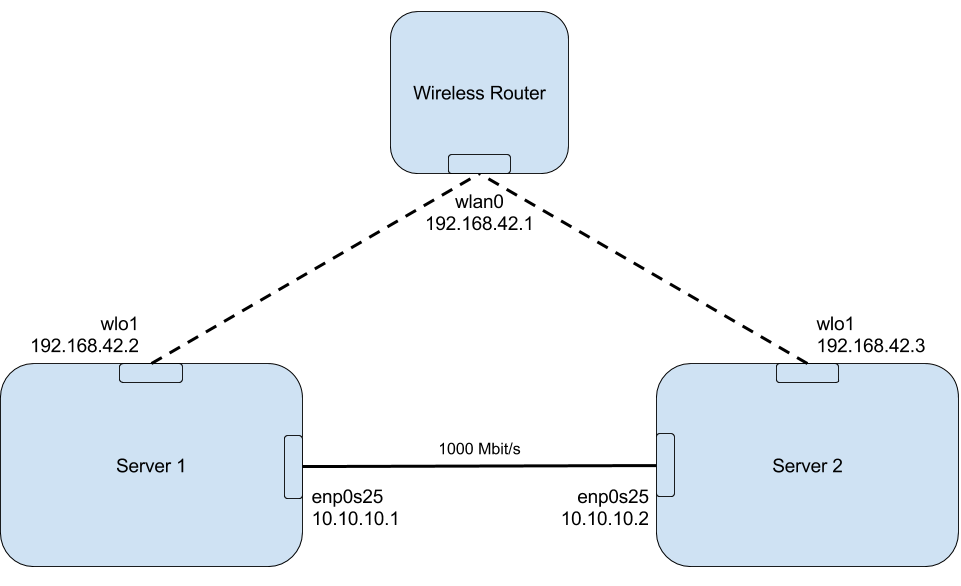
\includegraphics[width=10.5cm]{figure/labenv}
    \caption{Overview of Physical Lab}
    \label{fig:labenv}
\end{figure}

\skippara \cref{fig:vmenv} shows a virtual lab in Oracle VM VirtualBox (5.1.22) on a host with Intel(R) Core(TM) processor i5-5257U at 2.7 GHz, 8 GB memory, and macOS Sierra 10.12.5 operating system.
There are two \glspl{vm}, or guest \glspl{os}, on top of the host with similar settings, such as one processor, 2 GB base memory, Ubuntu Server 16.04.2 LTS (Xenial Xerus) operating system and Linux kernel version 4.4.0.

\skippara Also, each \gls{vm} has two virtio network interfaces.
First one connects to the host in \gls{nat}-mode to manage the \glspl{vm} via \acrshort{ssh}.
Moreover, the second interface connects the \gls{vm}s in ``internal networking''-mode.

\begin{figure}[h!]
    \centering
    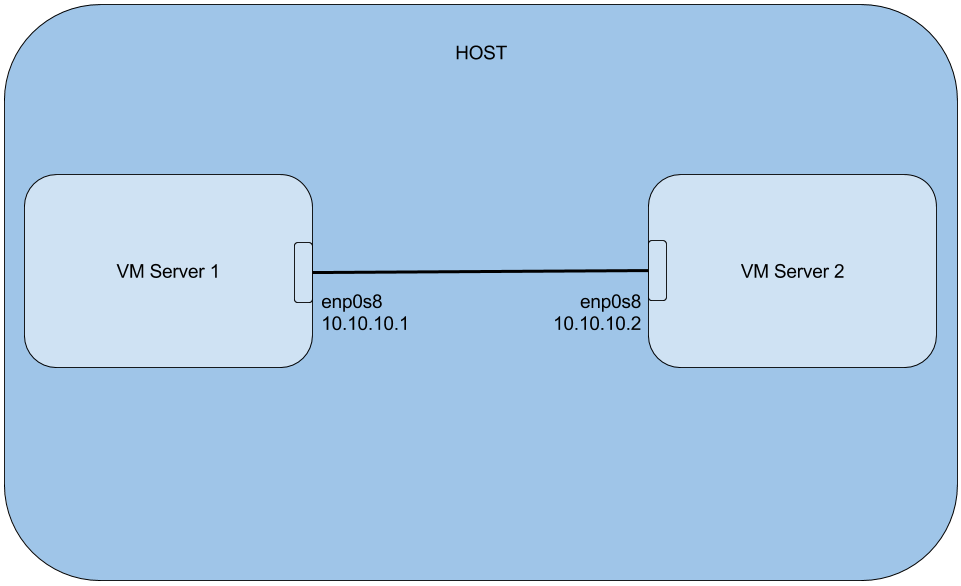
\includegraphics[width=10.5cm]{figure/vmenv}
    \caption{Overview of Virtual Lab}
    \label{fig:vmenv}
\end{figure}

%----------------------------------------------------------------
%
% Tools
%
%----------------------------------------------------------------
\hfill\break
\section{Tools}
We ran Docker (17.05.0-ce) on both of the servers to manage containers.
Then, used open source software, such as Iperf (2.0.9), Mausezahn (0.6.3) and Ostinato (0.8-1) to generate network traffic on the first server.
On the second server, we ran Tcpdump (4.9.0) to capture packets and Capinfos (2.2.6) to analyze captured packets.
Also, these tools were packaged or containerized, into five different Docker images.
For a more detailed look into the implementation, please see \cref{app:code} or \url{https://github.com/saimanwong/mastersthesis}.

\subsection{Iperf}
Iperf is available on Windows, Linux and BSD \cite{iperf2do7:online, iPerfThe63:online}.
This tool focuses on throughput testing rather than to craft packets.
Thus, Iperf supports only layer 3 and 4, such as \acrshort{tcp}, \acrshort{udp}, \acrshort{sctp}, \acrshort{ipv4}, and \acrshort{ipv6}.
Iperf uses a client-server architecture to analyze network traffic.
However, Iperf 3 does not support a serverless client to send \acrshort{udp} traffic \cite{Serverle80:online}.
Thus, we selected Iperf 2 for this project's purpose, and it can also run multiple threads.

\skippara The Iperf include the image \texttt{saimanwong/iperf}, as shown in \cref{code:iperf}.
It only required \gls{cli}-command to spin up this container for traffic generation.

\clearpage
\subsection{Mausezahn}
Mausezahn is only available for Linux and BSD \cite{netsniff7:online, UbuntuMa4:online}.
It is a tool to craft packets, generate and analyze network traffic.
Also, it supports protocols from layer 2 to 7.
Finally, it is possible to run Mausezahn in either ``direct'' or ``interactive'' mode.
The former craft packets direct via the \gls{cli} with multiple parameters.
The latter can create arbitrary streams of packets with its \gls{cli}.

\skippara The Mausezahn include the image \texttt{saimanwong/mausezahn}, as shown in \cref{code:mausezahn}.
It only required \gls{cli}-command in ``direct mode'' to spin up this container for traffic generation.


\subsection{Ostinato}
Ostinato is compatible with Windows, Linux, BSD and macOS \cite{Ostinato63:online, pstavirs92:online}.
This tool is similar to Mausezahn as it can craft, generate and analyze packets.
Also, Ostinato supports protocols from layer 2 to 7, for example, Ethernet/802.3, \acrshort{vlan}, \acrshort{arp}, \acrshort{ipv4}, \acrshort{ipv6}, \acrshort{tcp}, \acrshort{udp} and \acrshort{http} to only mention a few.
Its architecture consists of controller(s) and agent(s).
That is, it is possible to use either a \acrshort{gui} or Python \gls{api} as a controller to manage the agent and generate streams of packets from a single or several machines at the same time.

\skippara The Ostinato solution consists of the images \texttt{saimanwong/ostinato-drone} and \texttt{saimanwong/ostinato-python-api}, as shown in \cref{code:ostinato-drone} and \cref{code:ostinato-python-api} respectively.
The first image creates a container with an Ostinato agent that waits for instructions to generate packets.
Finally, the second image spins up a controller container to communicate with the agent via a Python script.

\subsection{Tcpdump and Capinfos}
Tcpdump uses the library libpcap, thus, works on Linux, BSD, and macOS \cite{TCPDUMPL66:online}.
Additionally, there is also a port called WinPcap \cite{WinPcapH61:online}.
Nevertheless, the usage of Tcpdump is to capture and analyze packets on a specified network interface.
These captured packets can then either be printed out on the terminal or saved to a file, usually ``.pcap''.
We then use the Wireshark's \gls{cli}-tool Capinfos to interpret the pcap-file in the form of statistics, such as the bit rate \cite{ToolsThe22:online}.

\skippara Tcpdump and Capinfos are combined into the image \texttt{saimanwong/tcpdump-capinfos}, as shown in \cref{code:tcpdump-capinfos}.
It is similar to the latter section, that is, to execute a \gls{cli}-command to capture and analyze packets.

%----------------------------------------------------------------
%
% Data Collection
%
%----------------------------------------------------------------
\clearpage
\section{Data Collection}\label{section:datacollection}
Similar to \cite{kolahi2011performance, srivastava2014evaluation, srivastava2014comparative}, we ran UDP throughput experiments with packet sizes that vary from 64 bytes to 4096 bytes.
That is, server 1 (source) sends packets over the link, and server 2 (sink) captures the packets.
Finally, for each packet size, we generate and capture packets for 10 seconds to get the throughput in \acrshort{mbps}.
We repeated it100 times to get a sample mean and standard deviation to understand the sparseness.

\skippara We evaluated Iperf, Mausezahn, and Ostinato in two different throughput experiments:
\begin{itemize}
    \item Experiment 1 -- Physical Hardware (\cref{fig:labenv})
    \item Experiment 2 -- Virtual Hardware (\cref{fig:vmenv})
\end{itemize}

\skippara Finally, \cref{eq:throughput} shows the theoretical limit of throughput over a link \cite{meyer2013measurement}.
$S$ represents packet size, and $\lambda$ the packet rate.
Each Ethernet frame includes a 7-byte preamble, a 1-byte start of frame delimiter and a 12-byte interframe gap.

\begin{equation}\label{eq:throughput}
    D_b = (S + 7B + 1B + 12B)*8\frac{Bit}{B}*\lambda
\end{equation}

\subsection{Settings}\label{section:settings}

\skippara In Iperf, it is only required to specify the source and destination \gls{ipv4} address since it tests either \acrshort{tcp} or \acrshort{udp} throughput.
\cref{iperfparam} shows the rest of the parameters for Iperf.

\skippara In Ostinato and Mausezahn, we build streams of packets up to transport layer (layer 4), such as \gls{mac}, Ethernet II, \gls{ipv4} and \gls{udp} respectively.
Thus, it is required to specify the \gls{mac} and \gls{ipv4} addresses for both the destination and source.
Also, to select the \gls{nic} to transmit packets.
\cref{ostinatoparam} and \cref{mausezahnparam} presents the remaining settings of Ostinato and Mausezahn respectively.


\begin{table}[ht!]
    \small
    \caption{Experiment Parameters -- Iperf}
    \label{iperfparam}
    \begin{adjustbox}{center}
        \renewcommand*\arraystretch{1.2}\begin{tabular}{| L{3.5cm} || L{4.5cm} |}
            \hline
            \textbf{Number of Packets} & Infinite
            \\ \hline
            \textbf{Bandwidth} & 1000 Mbps
            \\ \hline
            \textbf{Threads} & 1
            \\ \hline
            \textbf{Protocol} & \gls{udp}
            \\ \hline
            \textbf{Packet Size} & 64 - 4096
            \\ \hline
            \textbf{Experiment Time} & 10 seconds $\times$ 100 iterations
            \\ \hline
        \end{tabular}
    \end{adjustbox}
\end{table}


\begin{table}[ht!]
    \small
    \caption{Experiment Parameters -- Mausezahn}
    \label{mausezahnparam}
    \begin{adjustbox}{center}
        \renewcommand*\arraystretch{1.2}\begin{tabular}{| L{3.5cm} || L{4.5cm} |}
            \hline
            \textbf{Number of Packets} & Infinite
            \\ \hline
            \textbf{Protocol} & \gls{udp}
            \\ \hline
            \textbf{Packet Size} & 64 - 4096
            \\ \hline
            \textbf{Experiment Time} & 10 seconds $\times$ 100 iterations
            \\ \hline
        \end{tabular}
    \end{adjustbox}
\end{table}


\begin{table}[ht!]
    \small
    \caption{Experiment Parameters -- Ostinato}
    \label{ostinatoparam}
    \begin{adjustbox}{center}
        \renewcommand*\arraystretch{1.2}\begin{tabular}{| L{3.5cm} || L{4.5cm} |}
            \hline
            \textbf{Number of Bursts} & 1 000 000
            \\ \hline
            \textbf{Packets per Burst} & 10
            \\ \hline
            \textbf{Bursts per Second} & 50 000
            \\ \hline
            \textbf{Protocol} & \gls{udp}
            \\ \hline
            \textbf{Packet Size} & 64 - 4096
            \\ \hline
            \textbf{Experiment Time} & 10 seconds $\times$ 100 iterations
            \\ \hline
        \end{tabular}
    \end{adjustbox}
\end{table}

